\documentclass{dissertation}

\begin{document}

%% Specify the title and author of the thesis. This information will be used on
%% the title page (in title/title.tex) and in the metadata of the final PDF.
\title[Optional Subtitle]{Title}
\author{Albert}{Einstein}

%% Use Roman numerals for the page numbers of the title pages and table of
%% contents.
\frontmatter

\begin{titlepage}

\begin{center}

%% Extra whitespace at the top.
\vspace*{2\bigskipamount}

%% Print the title.
{\makeatletter
\titlestyle\singlespacing\bfseries\LARGE\@title\par
\makeatother}

%% Print the optional subtitle.
{\makeatletter
\ifx\@subtitle\undefined\else
    \bigskip
    \titlefont\titleshape\Large\@subtitle
\fi
\makeatother}

\end{center}

\cleardoublepage
\thispagestyle{empty}

\begin{center}

%% The following lines repeat the previous page exactly.

\vspace*{2\bigskipamount}

%% Print the title.
{\makeatletter
\titlestyle\singlespacing\bfseries\LARGE\@title\par
\makeatother}

%% Print the optional subtitle.
{\makeatletter
\ifx\@subtitle\undefined\else
    \bigskip
    \titlefont\titleshape\Large\@subtitle
\fi
\makeatother}


%% Uncomment the following lines to insert a vertically centered picture into
%% the title page.
%\vfill
%\includegraphics{title}
\vfill

%% Apart from the names and dates, the following text is dictated by the
%% promotieregelement.

{\Large\titlefont\bfseries Proefschrift}

\bigskip
\bigskip

ter verkrijging van de graad van doctor

aan de Technische Universiteit Delft,

op gezag van de Rector Magnificus prof.~???,

voorzitter van het College voor Promoties,

in het openbaar te verdedigen op dinsdag 1 Maart 2023 om 10:00 uur

\bigskip
\bigskip

door

\bigskip
\bigskip

%% Print the full name of the author.
\makeatletter
{\Large\titlefont\bfseries\@firstname\ {\titleshape\@lastname}}
\makeatother
\\
\vspace{3mm}
\begin{CJK*}{UTF8}{gkai}
\makeatletter
{\LARGE\titlefont\bfseries\@lastnameCH\ \hspace{1mm} {\titleshape\@firstnameCH}}
\makeatother
\end{CJK*}

\bigskip
\bigskip

Master of Science in Applied Physics,

Delft University of Technology, the Netherlands,

geboren te Hohhot, P.~R.~China.

%% Extra whitespace at the bottom.
\vspace*{2\bigskipamount}

\end{center}

\clearpage
\thispagestyle{empty}

%% The following line is dictated by the promotieregelement.
\noindent Dit proefschrift is goedgekeurd door de promotor:

%% List the promotors (supervisors).
\medskip\noindent
\begin{tabular}{l}
    Prof.\ dr.\ H.\ P.\ Urbach
\end{tabular}

%% List the (optional) copromotor.
\medskip
\noindent Copromotor: Dr.\ F.\ Bociort

\medskip
\noindent Samenstelling promotiecommissie:

%% List the committee members, starting with the Rector Magnificus and the
%% promotor(s) and ending with the reserve members.
\medskip\noindent
\begin{tabular}{ll}
    Rector Magnificus, & voorzitter \\
    Prof.\ dr.\ H.\ P.\ Urbach, & Technische Universiteit Delft, promotor \\
    Dr.\ F.\ Bociort, & Technische Universiteit Delft, copromotor \\
    ??? & ??? \\
    ??? & ??? \\
    ??? & ??? \\
    ??? & ??? \\
    ??? & ??? \\
\end{tabular}

%% Include the following disclaimer for committee members who have contributed
%% to this dissertation. Its formulation is again dictated by the
%% promotieregelement.
\medskip
\noindent Prof.\ dr.\ ir.\ ???.\ ??? heeft als begeleider in belangrijke mate aan de totstandkoming van het proefschrift bijgedragen.

%% Here you can include the logos of any institute that contributed financially
%% to this dissertation.
\vfill
\begin{center}
    
\includegraphics[height=0.6in]{title/logos/tudelftpng}
    \hspace{2em}
    
\includegraphics[height=0.6in]{title/logos/marie-curie}
    \hspace{2em}
    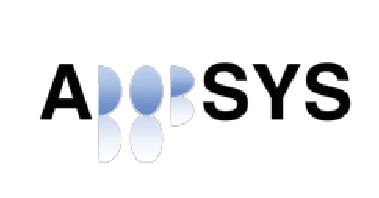
\includegraphics[height=0.55in]{title/logos/adopsys}
\end{center}
\vfill

\noindent
\begin{tabular}{@{}p{0.2\textwidth}@{}p{0.8\textwidth}}
    \textit{Keywords:} & \ldots \\[\medskipamount]
    \textit{Printed by:} & Johannes Gutenberg \\[\medskipamount]
    \textit{Front \& Back:} & Beautiful cover art that captures the entire content of this thesis in a single illustration.
\end{tabular}

\vspace{4\bigskipamount}

\noindent Copyright \textcopyright\ 2022 by Zhe Hou

%% Uncomment the following lines if this dissertation is part of the Casimir PhD
%% Series, or a similar research school.
%\medskip
%\noindent Casimir PhD Series, Delft-Leiden 2013-01

\medskip
\noindent ISBN 000-00-0000-000-0

\medskip
\noindent An electronic version of this dissertation is available at \\
\url{http://repository.tudelft.nl/}.

\newpage
\;
\vspace{12em}



% Here is the explanation about the cover
\begin{figure}[h!]
    \centering
    
\includegraphics[scale=0.35]{cover/CoverSP.png}
\end{figure} 
Designed by Hui Lin

 The concept is borrowed from Escher's style. We draw horse patterns together with the "saddle" which relates to the "saddle point". In between the horse patterns, there are pieces of convex and concave lens shape. I would like to indicate a lens design network or space that the lens solutions are linked/surrounded by saddles (saddle points). In a whole, with Escher's way of presenting, the pattern seems quite complicated, yet is composed with a monotonic repetitive pattern (the feeling of the complexity is probably from the color composition and angular arrangement). It is sort of related to the goal of the thesis/research: in a complicated design landscape, we are trying to find a systematic way to describe it and then utilize knowledge for practical design. 

\end{titlepage}



%% The (optional) dedication can be used to thank someone or display a
%% significant quotation.
\dedication{\epigraph{Science is a wonderful thing \\ if one does not have to earn one's living at it.}{Albert Einstein}}

\chapter*{Preface}
\setheader{Preface}

Preface\ldots

\begin{flushright}
\LARGE\textbf{unnecessary}
{\makeatletter\itshape
    \@firstname\ \@lastname \\
    Delft, January 2013
\makeatother}
\end{flushright}



\tableofcontents

%% Use Arabic numerals for the page numbers of the chapters.
\mainmatter

%% Turn on thumb indices.
\thumbtrue

\chapter{Introduction}
\label{chapter_1}

%% The following annotation is customary for chapter which have already been
%% published as a paper.
\blfootnote{Parts of this chapter have been published in Annalen der Physik \textbf{324}, 289 (1906) \cite{Einstein1906}.}

%% It is only necessary to list the authors if multiple people contributed
%% significantly to the chapter.
\authors{Albert {\titleshape Einstein}}

%% The '0pt' option ensures that no extra vertical space follows this epigraph,
%% since there is another epigraph after it.
\epigraph[0pt]{
    Nature and nature's laws lay hid in the night; \\
    God said `Let Newton be!' and all was light.
}{Alexander Pope}

\epigraph{
    It did not last: the devil shouting `Ho. \\
    Let Einstein be!' restore the status quo.
}{Sir John Collings Squire}

\begin{abstract}
Lorem ipsum dolor sit amet, consectetur adipisicing elit, sed do eiusmod tempor incididunt ut labore et dolore magna aliqua. Ut enim ad minim veniam, quis nostrud exercitation ullamco laboris nisi ut aliquip ex ea commodo consequat. Duis aute irure dolor in reprehenderit in voluptate velit esse cillum dolore eu fugiat nulla pariatur. Excepteur sint occaecat cupidatat non proident, sunt in culpa qui officia deserunt mollit anim id est laborum.
\end{abstract}

%% Start the actual chapter on a new page.
\newpage

\noindent This document is intended to be both an example of the TU Delft dissertation template for \LaTeX, as well as a short introduction to its use. It is not intended to be a general introduction to \LaTeX{} itself,\footnote{We recommend \url{http://en.wikibooks.org/wiki/LaTeX} as a reference and a starting point for new users.} and we will assume the reader to be familiar with the basics of creating and compiling documents.

Instructions on how to use this template under Windows and Linux, and which \LaTeX{} packages are required, can be found in \texttt{README.txt}.

%%%%%%%%%%%%%%%%%%%%%%%%%% SECTION 1 %%%%%%%%%%%%%%%%%%%%%%%%%%%%%%%%%%%%%%%%%%%%%%%%%%%%%%%%
\section{Problem for optical system design}
\vspace{1em}
How does this nonlinearty appear?

%% We need an empty line before the quote environment to work around a bug in
%% the lettrine package, from which the drop command is derived.
\begin{quote}
\texttt{\textbackslash documentclass\{dissertation\}}
\end{quote}
which loads the dissertation template. The template is based on the \LaTeX{} \texttt{book} document class and stored in \texttt{dissertation.cls}. The document class accepts several comma-separated options. By default, hyperlinks are shown in cyan, which is convenient when reading the dissertation on a computer, but can be expensive when printing. They can be turned black with the \texttt{print} option. This will also turn the headers dark gray instead of cyan. Moreover, it will add a 3~mm bleed around the page including crop marks. This will help the printer with the thumb indices, since they run right up to the page borders. Finally, the \texttt{nativefonts} option can be used to override the automatic font selection (see below).

A dissertation is a big document, which makes it easy to miss warnings about the layout in the \LaTeX{} output. In order to locate problem areas, add the \texttt{draft} option to the \texttt{\textbackslash documentclass} line. This will display a vertical bar in the margins next to the paragraphs that require attention.

The contents of the dissertation are included between the \texttt{\textbackslash begin\{document\}} and \texttt{\textbackslash end\{document\}} commands, and split into three parts by
\begin{enumerate}
\item\texttt{\textbackslash frontmatter}, which uses Roman numerals for the page numbers and is used for the title page and the table of contents;
\item\texttt{\textbackslash mainmatter}, which uses Arabic numerals for the page numbers and is the style for the chapters;
\item\texttt{\textbackslash appendix}, which uses letters for the chapter numbers, starting with `A'.
\end{enumerate}
The title page is defined in \texttt{title.tex} in the \texttt{title} folder and included verbatim with \texttt{\textbackslash include\{title/title\}},\footnote{Note that it is not necessary to specify the file extension.} (see below). Additionally, it is possible to include a preface, containing, for example, the acknowledgements. An example can be found in \texttt{preface.tex}. The table of contents is generated automatically with the \texttt{\textbackslash tableofcontents} command. Chapters are included after \texttt{\textbackslash mainmatter} and appendices after \texttt{\textbackslash appendix}. For example, \texttt{\textbackslash include\{chapter-1/chapter-1\}} includes \texttt{chapter-1.tex}, which contains this introduction.

%%%%%%%%%%%%%%%%%%%%%%%%%% SECTION 2 %%%%%%%%%%%%%%%%%%%%%%%%%%%%%%%%%%%%%%%%%%%%%%%%%%%%%%%%
\section{Traditional lens design strategy}
\vspace{1em}
Example of traditional lens design strategy to find alternative solutions.

\dropcap{T}{he} title pages are defined in \texttt{title/title.tex}, which you will have to modify according to your needs. Note that these pages are subject to the requirements of the \emph{promotieregelement} and cannot be changed at will. Apart from the names and dates, most of the Dutch text is dictated literally.

Since the thesis title and name of the author appear several times throughout the document (on the title page, but also in, \emph{e.g.}, the preface and cv), special commands are provided so they only have to be specified once. The title (and optional subtitle) can be specified with

\begin{quote}
\texttt{\textbackslash title[Optional subtitle]\{Title\}}
\end{quote}
The name of the author is specified with
\begin{quote}
\texttt{\textbackslash author\{First name\}\{Last name\}}
\end{quote}
Note that the first and last name are separate arguments, since they may be printed in different font shapes. The \texttt{\textbackslash title} and \texttt{\textbackslash author} commands also ensure that the title and author appear in the metadata of the final PDF.

See \texttt{title/title.tex} for detailed documentation on the comment and layout of the title pages. Logos of institutes that have contributed financially to the dissertation may be included on reverse side of the title page. A few example logos can be found in the \texttt{title/logos} folder.

%%%%%%%%%%%%%%%%%%%%%%%%%% SECTION 3 %%%%%%%%%%%%%%%%%%%%%%%%%%%%%%%%%%%%%%%%%%%%%%%%%%%%%%%%
\section{Lens optimizations local\&global}

\dropcap{E}{ach} chapter has its own file. For example, the \LaTeX{} source of this chapter can be found in \texttt{chapter-1.tex}. A chapter starts with the command

\begin{quote}
\texttt{\textbackslash chapter\{Chapter title\}}
\end{quote}
This starts a new page, prints the chapter number and title and adds a link in the table of contents. If the title is very long, it may be desirable to use a shorter version in the page headers and the table of contents. This can be achieved by specifying the short title in brackets:

\begin{quote}
\texttt{\textbackslash chapter[Short title]\{Very long title with many words which could not possibly fit on one line\}}
\end{quote}
Unnumbered chapters, such as the preface, can be created with \texttt{\textbackslash chapter*\{Chapter title\}}. Such a chapter will not show up in the table of contents or in the page header. To create a table of contents entry anyway, add
\begin{quote}
    \texttt{\textbackslash addcontentsline\{toc\}\{chapter\}\{Chapter title\}}
\end{quote}
after the \texttt{\textbackslash chapter} command. To print the chapter title in the page header, add
\begin{quote}
    \texttt{\textbackslash setheader\{Chapter title\}}
\end{quote}

If (parts of) the chapter have already been published elsewhere, it is customary to add a reference. This can be done with the special unnumbered footnote command \texttt{\textbackslash blfootnote}. For example,

\begin{quote}
\texttt{\textbackslash blfootnote\{Parts of this chapter have been published in Annalen der Physik \textbackslash textbf\{324\}, 289 (1906) \textbackslash cite \{Einstein1906\}.\}}
\end{quote}
generates the footnote at the beginning of this chapter. Because this footnote is unnumbered, the \texttt{hyperref} package may throw a warning, which safely be ignored.

If multiple people have contributed significantly to this chapter, they can be lister with the \texttt{\textbackslash authors} command. This can be followed by a quotation using \texttt{\textbackslash epigraph} as shown above. Finally, it is customary for a dissertation to include an abstract for every chapter (except perhaps the introduction). This can be accomplished with the \texttt{abstract} environment. The abstract should be followed by \texttt{\textbackslash newpage} to start the chapter text on a new page.

In a dissertation, each chapter has its own list of references. These can be generated with the special command \texttt{\textbackslash references\{dissertation\}} from \texttt{dissertation.bib} at the end of the chapter. Note that this means that you need to run a command like \texttt{bibtex chapter-1/chapter-1} for each chapter. The bibliography style is specified in \texttt{dissertation.bst}, which is a modified version of \texttt{apsrev4-1.bst} (from REVTeX) designed to also display the titles of referenced articles. The template will automatically generate clickable hyperlinks if a URL or DOI (digital object identifier) is present for the reference. Although it is possible to manage the bibliography by hand, we recommend using EndNote (available from Blackboard) or JabRef (available from \url{http://jabref.sourceforge.net/}).

Chapters are subdivided into sections, subsections, subsubsections, and, optionally, paragraphs and subparagraphs. All can have a title, but only sections and subsections are numbered. As with chapters, the numbering can be turned off by using \texttt{\textbackslash section*\{\ldots\}} instead of \texttt{\textbackslash section\{\ldots\}}, and similarly for the subsection.

%%%%%%%%%%%%%%%%%%%%%%%%%% SECTION 4 %%%%%%%%%%%%%%%%%%%%%%%%%%%%%%%%%%%%%%%%%%%%%%%%%%%%%%%%
\section{Other design strategy?}
\subsection{\textbackslash subsection\{\ldots\}}
\subsubsection{\textbackslash subsubsection\{\ldots\}}
\paragraph{\textbackslash paragraph\{\ldots\}}
Lorem ipsum dolor sit amet, consectetur adipisicing elit, sed do eiusmod tempor incididunt ut labore et dolore magna aliqua. Ut enim ad minim veniam, quis nostrud exercitation ullamco laboris nisi ut aliquip ex ea commodo consequat. Duis aute irure dolor in reprehenderit in voluptate velit esse cillum dolore eu fugiat nulla pariatur. Excepteur sint occaecat cupidatat non proident, sunt in culpa qui officia deserunt mollit anim id est laborum.

%%%%%%%%%%%%%%%%%%%%%%%%%% SECTION 5 %%%%%%%%%%%%%%%%%%%%%%%%%%%%%%%%%%%%%%%%%%%%%%%%%%%%%%%%
\section{Goal of this thesis}

\dropcap{T}{he} fonts used by this template depend on which version of \LaTeX{} you use. Regular \LaTeX, \emph{i.e.}, if you compile your document with with \texttt{latex}, \texttt{pslatex} or \texttt{pdflatex}, will use Utopia for text, Fourier for math and Latin Modern for sans-serif and monospaced text. However, if you want to adhere to the TU Delft house style, you will need to use \XeLaTeX, as it supports TrueType and OpenType fonts. Compiling with \texttt{xelatex} will use Bookman Old Style for titles, Tahoma for text, Courier New for monospace and Cambria for math. If you want to use \XeLaTeX, but do not want to use the TU Delft house style fonts, you can add the \texttt{nativefonts} option to the document class.

This template supports the use of drop caps, a large colored initial at the beginning of a chapter or section, via the \texttt{\textbackslash dropcap} command:

\begin{quote}
\texttt{\textbackslash dropcap\{L\}\{orem\} ipsum\ldots}
\end{quote}
The first argument is the capital that will be printed on two lines (in the title color), and the second argument is the rest of the word. Depending on the font, the latter may be printed in small caps.

The corporate colors of the TU Delft are cyan, black and white, available, respectively, via \texttt{\textbackslash color\{{\color{tudelft-cyan}tudelft-cyan}\}}, \texttt{\textbackslash color\{{\color{tudelft-black}tudelft-black}\}} (which differs slightly from the default \texttt{black}) and \texttt{\textbackslash color\{tudelft-white\}}. Apart from these three, the house style defines the basic colors
\begin{itemize}
%% Reduce the separation between the items, since this is just a list of words.
\itemsep 0pt
\parskip 0pt
\item\texttt{\color{tudelft-sea-green}tudelft-sea-green},
\item\texttt{\color{tudelft-green}tudelft-green},
\item\texttt{\color{tudelft-dark-blue}tudelft-dark-blue},
\item\texttt{\color{tudelft-purple}tudelft-purple},
\item\texttt{\color{tudelft-turquoise}tudelft-turquoise} and
\item\texttt{\color{tudelft-sky-blue}tudelft-sky-blue},
\end{itemize}
as well as the accent colors
\begin{itemize}
\itemsep 0pt
\parskip 0pt
\item\texttt{\color{tudelft-lavendel}tudelft-lavendel},
\item\texttt{\color{tudelft-orange}tudelft-orange},
\item\texttt{\color{tudelft-warm-purple}tudelft-warm-purple},
\item\texttt{\color{tudelft-fuchsia}tudelft-fuchsia},
\item\texttt{\color{tudelft-bright-green}tudelft-bright-green} and
\item\texttt{\color{tudelft-yellow}tudelft-yellow}.
\end{itemize}

\references{dissertation}


\chapter{The Saddle Point Construction Method}
\label{chapter_2}
\graphicspath{ {./chapter-sp/figures/} }
\captionsetup[figure]{labelfont=bf}
\captionsetup{margin=1.5em}
\captionsetup[table]{labelfont=bf}
%% The following annotation is customary for chapter which have already been
%% published as a paper.


%% It is only necessary to list the authors if multiple people contributed
%% significantly to the chapter.
%\authors{Albert {\titleshape Einstein}}

%% The '0pt' option ensures that no extra vertical space follows this epigraph,
%% since there is another epigraph after it.

\begin{abstract}
The saddle point construction method is elaborated in this chapter. Recommendations on how to apply the method are given based on simple examples.
\end{abstract}

%% Start the actual chapter on a new page.
\newpage

\noindent 
The saddle point construction (SPC) method is one of the major methods investigated in this research. Several variations of the methods for constructing the saddle point system have been introduced through the years \cite{BociortSPCSexplained}\cite{MVTurnhoutSPC15}\cite{HouProc2015}. Instead of searching for alternative local minima, the SPC method constructs saddle points as intermediate steps to obtain new local minima. This is achieved by adding extra variables to the existing system. With this approach, it is shown in this chapter that it is possible to obtain new solutions in a systematic way. 

%%%%%%%%%%%%%%%%%%%%%%%%%%%%%%%%%%%%%%%%%%%%%%% Section SPC %%%%%%%%%%%%%%%%%%%%%%%%%%%%%%%%%%%%%%%%%%%%%
\section{Saddle point and design landscape}
For a given optical design problem, once the merit function and the number of variables N have been determined, an N-dimensional design (optimization) space is defined. The optimization of an optical system then is equivalent to finding the minimum of the merit function in the N-dimensional design landscape. As mentioned in the introduction, the optimization problem of optical design is a nonlinear problem, where multiple local minima are present in the design landscape. As a result, searching for one or several good local minima among many becomes a challenge for optical design. 

For the simple case of only two variables, the minima can be viewed as the bottoms of the valleys in the design landscape. On the other hand, maxima are the mountain tops, which are usually not observed in the lens design landscape. Minima and maxima are both critical points. A critical point is a point where the gradient of the merit function equals zero. In addition to minima and maxima, there are saddle points, which are also critical points and can be used to find new local minima.

In a two dimensional space, a 2-D saddle point is a "saddle" where along one direction in variable space, the value of the function decreases with respect to the saddle point value, while along the perpendicular direction, it increases. Mathematically, the so-called Morse Index is used to distinguish minima, maxima and saddle points. The Morse Index is defined as the number of negative eigenvalues of the Hessian matrix \textbf{$H$} at the critical point, when the Hessian matrix \textbf{$H$} is non-degenerate. A negative eigenvalue indicates that along the direction defined by the corresponding eigenvector of the Hessian matrix, the critical point is a maximum. Therefore, in an N-dimensional space, the Morse Index of a minimum and a maximum is 0 and N respectively. A saddle point can have any Morse Index between 1 and N-1. 

In this research, the saddle point with a Morse Index of 1 is of particular interest. This kind of saddle point has one direction, along which the value of the merit function decreases, while in N-1 other directions the merit function increases. This means that a saddle point of Morse Index 1 is a local minimum in all but one direction. When the optimization follows the two opposite directions in which the merit function descends, two local minima can in principle be found (Figure \ref{fig:SPCdemo}-b). As a result, if there is a way to rapidly obtain these saddle points in the design landscape, it provides an approach to find more local minima. In fact one finds two local minima from a saddle point of Morse Index 1. 

\section{The Saddle Point Construction method}
In this section, the SPC method and its variations are introduced and explained. As the name suggests, the method constructs saddle points in the design landscape. These are all saddle points with Morse Indices of $1$  \footnote{In the special version of the SPC, it can be proven that the Morse Index of the constructed saddle point is $1$. In the general version of the SPC, it is shown in the numerical experiments that the Morse Index of the constructed saddle point is $1$}. Instead of optimizing from an arbitrary point in the landscape, optimizing from a saddle point can systematically lead to two local minima. 

The saddle points are constructed by adding extra variables to the merit function that has attained the existing local minimum using the original number of variables. In principle, the variables can be any parameter in the lens design model. It should be mentioned that the most effective variables that have been used so far are the lens curvatures. 

\subsection{The general version of Saddle Point Construction \label{spc-general}}
\label{SPC_general}
The SPC method always starts with an optimized lens system that is a minimum of a merit function defined by N arbitrary variables. A saddle point then can be constructed in a design space with $N + 2$ variables by adding a lens with zero thickness and with surfaces having the same curvatures (see Figure \ref{fig:SPCdemo}(a)). Such a lens has no optical effect and hence the merit function is the same after insertion of this element as before. The two curvatures are the two new variables, so that the total number of variables has been increased to N+2. For certain values of the curvatures of the inserted surfaces, the resulting system is a saddle point, which is a minimum along $N + 1$ directions in the variable space and a maximum along one direction (i.e., mathematically it will have a Morse index of 1 \cite{MVTurnhoutSPC15}). The details of how such values are obtained will be explained in the part later. Along the direction for which the SP is a maximum, two minima can be obtained systematically, as shown for simplicity in a 2D case in Figure \ref{fig:SPCdemo}(b).

\begin{figure}[h!]
    \centering
    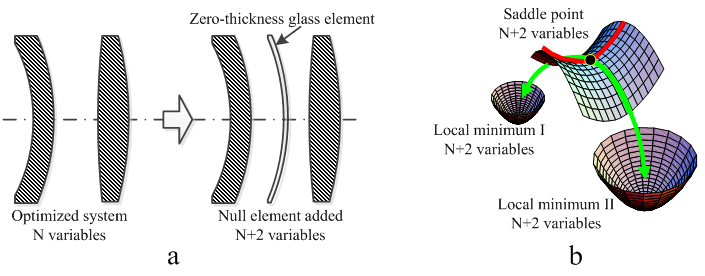
\includegraphics[scale=0.68]{chapter-2/figures/FigSPCDemo.png}
    \caption{Illustration of the SPC. (a) An SP in N+2 dimensional space obtained by insertion of a zero-thickness glass meniscus. (b) A Morse index 1 saddle point in the 2D case.}
    \label{fig:SPCdemo}
\end{figure}

The pair of surfaces with equal curvatures can be either a zero-thickness lens added to the original minimum or a zero-thickness air space inside a lens. Both the added lens and the added air space with zero thickness, do not affect the ray paths, and hence the merit function value of the original system is not changed. Such an element of zero thickness is therefore called a null element. 
Given the merit function $MF$ at a local minimum in $N$ dimensional space
\begin{equation}
MF^{N}(x^{0}_1, x^{0}_{2},...,x^{0}_{N}),
\end{equation}we have 
\begin{equation}\label{eq_mflm}
\frac{\partial}{\partial{x_i}}MF^{N}(x^{0}_1, x^{0}_{2},...,x^{0}_{N}) = 0, \;\; \text{for} \; i =1,2,...,N.
\end{equation}Furthermore the Morse Index of the Hessian at $(x^{0}_1, x^{0}_{2},...,x^{0}_{N})$ is zero, i.e. the eigenvalues of the matrix
\begin{equation}
H^{N}_{ij}=\frac{\partial^2}{\partial{x_i}\partial{x_j}} MF^{N}(x^{0}_1, x^{0}_{2},...,x^{0}_{N}),
\end{equation}are all non-negative.

Next we introduce a null element with common curvature $c_1=c_2$ of its two surfaces. Additional variables are then introduced as follows:

\begin{equation}
\begin{align}
\begin{rcases*}
x_{N+1} &= c_1 + c_2, \;\;\\
x_{N+2} &= c_1 - c_2. \;\;
\end{rcases*}
\end{align}
\end{equation}

Because the introduction of the null-element does not alter the physical property of the optical system, therefore does not have any effect on the merit function, we have the following relation between the $N$ and $N+2$ dimensional merit functions:
\begin{equation} \label{eq_mfconst}
MF^{N+2}(x_1, x_{2},...,x_{N}, x_{N+1},x_{N+2}=0) = MF^{N}(x_1, x_{2},...,x_{N}).
\end{equation}%because the variables are introduced in a way that the physical property of the optical system is not altered with the null-element. Therefore, the value of the merit function stays constant. 
%for some $(x_1, x_{2},...,x_{N-2})$ in some (sufficiently small) neighbourhood of  $(x^{0}_1, x^{0}_{2},...,x^{0}_{N-2})$ and all $x_{N-1}$. 
%Equation \ref{eq_mfconst} together with Equation \ref{eq_mflm} implies

Equation \ref{eq_mflm} implies
\begin{equation}
\begin{split}
\frac{\partial}{\partial{x_j}}MF^{N+2}&(x^{0}_1, x^{0}_{2},...,x^{0}_{N},x_{N+1},x_{N+2}=0) \\
&= \frac{\partial}{\partial{x_j}}MF^{N}(x^{0}_1, x^{0}_{2},...,x^{0}_{N}) \\
&= 0, \\
\text{for all} \: &j = 1, 2, ..., N, \:\: \text{and all} \:\: x_{N+1}.
\end{split}
\end{equation}Furthermore Equation \ref{eq_mfconst} implies 
\begin{equation}\label{MF_xn-1_fozero}
\frac{\partial}{\partial{x_{N+1}}}MF^{N+2}(x_1, x_{2},\cdots,x_{N}, x_{N+1},x_{N+2}=0) = 0,
\end{equation}%for all $(x_1, x_{2},...,x_{N-2})$ in a neighbourhood of $(x^{0}_1, x^{0}_{2},\cdots,x^{0}_{N-2})$ and 
for all $x_{N+1}$. 
Equation \ref{MF_xn-1_fozero} applies to $(x^{0}_1, x^{0}_{2},...,x^{0}_{N})$, we have
\begin{equation}
\begin{split}
\frac{\partial}{\partial{x_{N+1}}}MF^{N+2}&(x^0_1, x^0_{2},...,x^0_{N}, x_{N+1},x_{N+2}=0) = 0,\\
&\text{for all}\; x_{N+1}.
\end{split}
\end{equation}Next we vary $x_{N+1}$ to find a point $x^0_{N+1}$ for which 
\begin{equation}\label{eq:1dsearch}
\frac{\partial}{\partial{x_{N+2}}}MF^{N+2}(x^0_1, x^0_{2}, \cdots,x^0_{N}, x^0_{N+1},x_{N+2}=0) = 0.
\end{equation}Assuming that such point $x^0_{N+1}$ can be found, we conclude that 
\newline

\centerline{$(x^0_1, x^0_{2},\cdots,x^0_{N}, x^0_{N+1},0)$} 
\newline \noindent is a critical point of $MF^{N+2}$. 
 
Now Equation \ref{eq_mfconst} implies
\begin{equation}
\begin{split}
\frac{\partial}{\partial{x_i}\partial{x_j}}MF^{N+2}&(x^{0}_1, x^{0}_{2},...,x^{0}_{N},x^{0}_{N+1},x_{N+2}=0) \\
&= \frac{\partial}{\partial{x_i}\partial{x_j}}MF^{N}(x^{0}_1, x^{0}_{2},...,x^{0}_{N}), \\
\text{for} \;\;&\; 1\leq i,j \leq N.
\end{split}
\end{equation}Furthermore, from Equation \ref{MF_xn-1_fozero}
\begin{equation}
\begin{split}
\frac{\partial}{\partial{x_i}\partial{x_{N+1}}}MF^{N+2}&(x^{0}_1, x^{0}_{2},...,x^{0}_{N},x^{0}_{N+1},x_{N+2}=0) = 0, \;\; \\
\text{for all} & \;1\leq i \leq N+1.
\end{split}
\end{equation}
So we have for the Hessian in \textit{N+2} dimensional space
\begin{equation}\label{eq: the hessian}
\left( H^{N+2}_{ij} \right) = 
\begin{bmatrix}
\Large{\left( H^N_{ij} \right)}       &                 &   0                  & \frac{\partial{^2MF^{N+2}}}{\partial{x_1}\partial{x_{N+2}}} \\[2em]
                                                    &                 & \vdots         & \vdots \\[2em]
 0                                                 & \cdots    & 0                  & \frac{\partial{^2MF^{N+2}}}{\partial{x_{N+1}\partial{x_{N+2}}}}  \\[2em]
 \frac{\partial{^2MF^{N+2}}}{\partial{x_{N+2}}\partial{x_1}}   &\cdots  & \frac{\partial{^2MF^{N+2}}}{\partial{x_{N+2}}\partial{x_{N+1}}} & \frac{\partial{^2MF^{N+2}}}{\partial{x^2_{N+2}}}
\end{bmatrix}.
\end{equation}The last column and last row are in general nonzero, hence there are in general nonzero eigenvalues.
The eigenvalues of $H^{N}_{ij}$ are similar to a subset of $N$ eigenvalues of $H^{N+2}_{ij}$, but they are not the same. Nevertheless, it may be expected that they have the same sign, i.e. they are positive for

\vspace{0.1em}
\centerline {$(x^0_1, x^0_{2},\cdots,x^0_{N}, x^0_{N+1},0)$.}
\vspace{0.5em}

The question still remains what the sign is of the remaining two eigenvalues, because these signs determine the Morse Index at point $(x^{0}_1, x^{0}_{2},...,x^{0}_{N},x^{0}_{N+1},0)$.
\vspace{0.3em}

In practice, what has been observed so far in the SPC is that there are one positive sign and one negative sign. That means the point is a saddle point with Morse Index value of $1$. 

Obtaining saddle point systems with the general version of the SPC includes the following steps:
\begin{enumerate}[nosep] \label{para: performing SPC scan}
\item Insert a null element into the existing minimum.
\item Compute the derivative (numerically) of the merit function with respect to the curvature of the inserted null element. The null element has two identical curvatures. The computed derivative of the two curvatures have opposite sign. 
\item Select the curvature values where the derivative of the merit function equals zero. Systems with these curvature values are the saddle point systems. 
\end{enumerate}
These steps are referred as "performing an SPC scan" in this thesis.  In our research, the SPC scans are performed in CODE V using the MACRO function. Figure \ref{fig:SPCscan} shows an example of the results of such an SPC scan. An SPC scan in a chosen position can lead to multiple saddle point systems.  There are four zero crossings in Figure \ref{fig:SPCscan}(b) indicating that four saddle points are found. When the saddle points are found, initial systems for subsequent local optimization can be obtained by choosing for each zero crossing in Figure \ref{fig:SPCscan}(b) two systems, one to the left, one to the right of the saddle point. Local optimization, using, e.g., a damped-least square (DLS) algorithm, will then lead to two minima, one on each side of the “saddle,” as shown in Fig \ref{fig:SPCdemo}(b). To obtain the broadest variety of new minima with SPC, in general both zero-thickness lenses and zero-thickness air spaces are necessary. For simple systems, there are examples of minima that can be obtained with one of these two types of null elements but not with the other one. Finding the saddle points is in principle much less time consuming than DLS optimization, because it only involves the evaluation of the derivative of the MF for the 1D sequence of scan points according to Equation \ref{eq:1dsearch}, whereas local optimization involves many iterations where a Jacobian matrix is evaluated. The zero-thickness condition for the null element is not a severe limitation, as it may seem, because in the resulting minima the distances between the surfaces (and the glass of the new lens) can be easily changed as desired. Once the two local minima are obtained with the SPC, other parameters of the new lens (thickness, aspheric coefficients, etc.) can be made available as variables to further minimize the merit function.

\begin{figure}[h!]
    \centering
    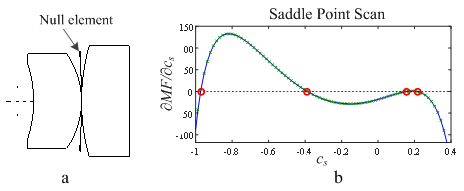
\includegraphics[scale=0.8]{chapter-2/figures/SPCscan.png}
    \caption{Example of an SPC scan. (a) The insertion of a glass null element between two lenses exhibiting a known minimum value of the merit function. (b) The SPC scan finds four saddle points in this search. The red circles indicate the corresponding values of the null element curvatures.}
    \label{fig:SPCscan}
\end{figure}

\subsection{The special version of Saddle Point Construction}
\label{SPC_Special}
Different from performing a scan using the general version of the SPC, the special version of the SPC directly constructs the saddle points by adding null elements to the existing system. This kind of null element (a glass or an air element) has to be attached to one of the existing surfaces in the system. The two curvatures of the null element have to be the same as that of the surface in contact. In such a case, three surfaces have the same curvatures and two zero-thickness spaces between them as illustrated in Figure \ref{fig:SPCS-illus}. It is explained in the previous section that such a constructed system can be a saddle point system with a Morse Index of either $1$ or $2$ (one negative eigenvalues or two negative eigenvalues from the remaining two for the Hessian matrix shown in Equation \ref{eq: the hessian}). In practice, we have not observed any case with a Morse Index of $2$ in our numerical experiment. When an equality constraint \footnote{For an optimization problem $min f(\mathbf{x})$, an equality constraint means that the problem is subject to $g_{equa}(\mathbf{x})=C_1$. An example of an inequality constraint can be that the problem is subject to $g_{inequa}(\mathbf{x}) > C_2$.} (e.g. a constraint on effective focal length) is applied to the system, it can be proven that such a saddle point system has a Morse Index of $1$ \cite{BociortSPCSexplained}.

\begin{figure}[h!]
    \centering
    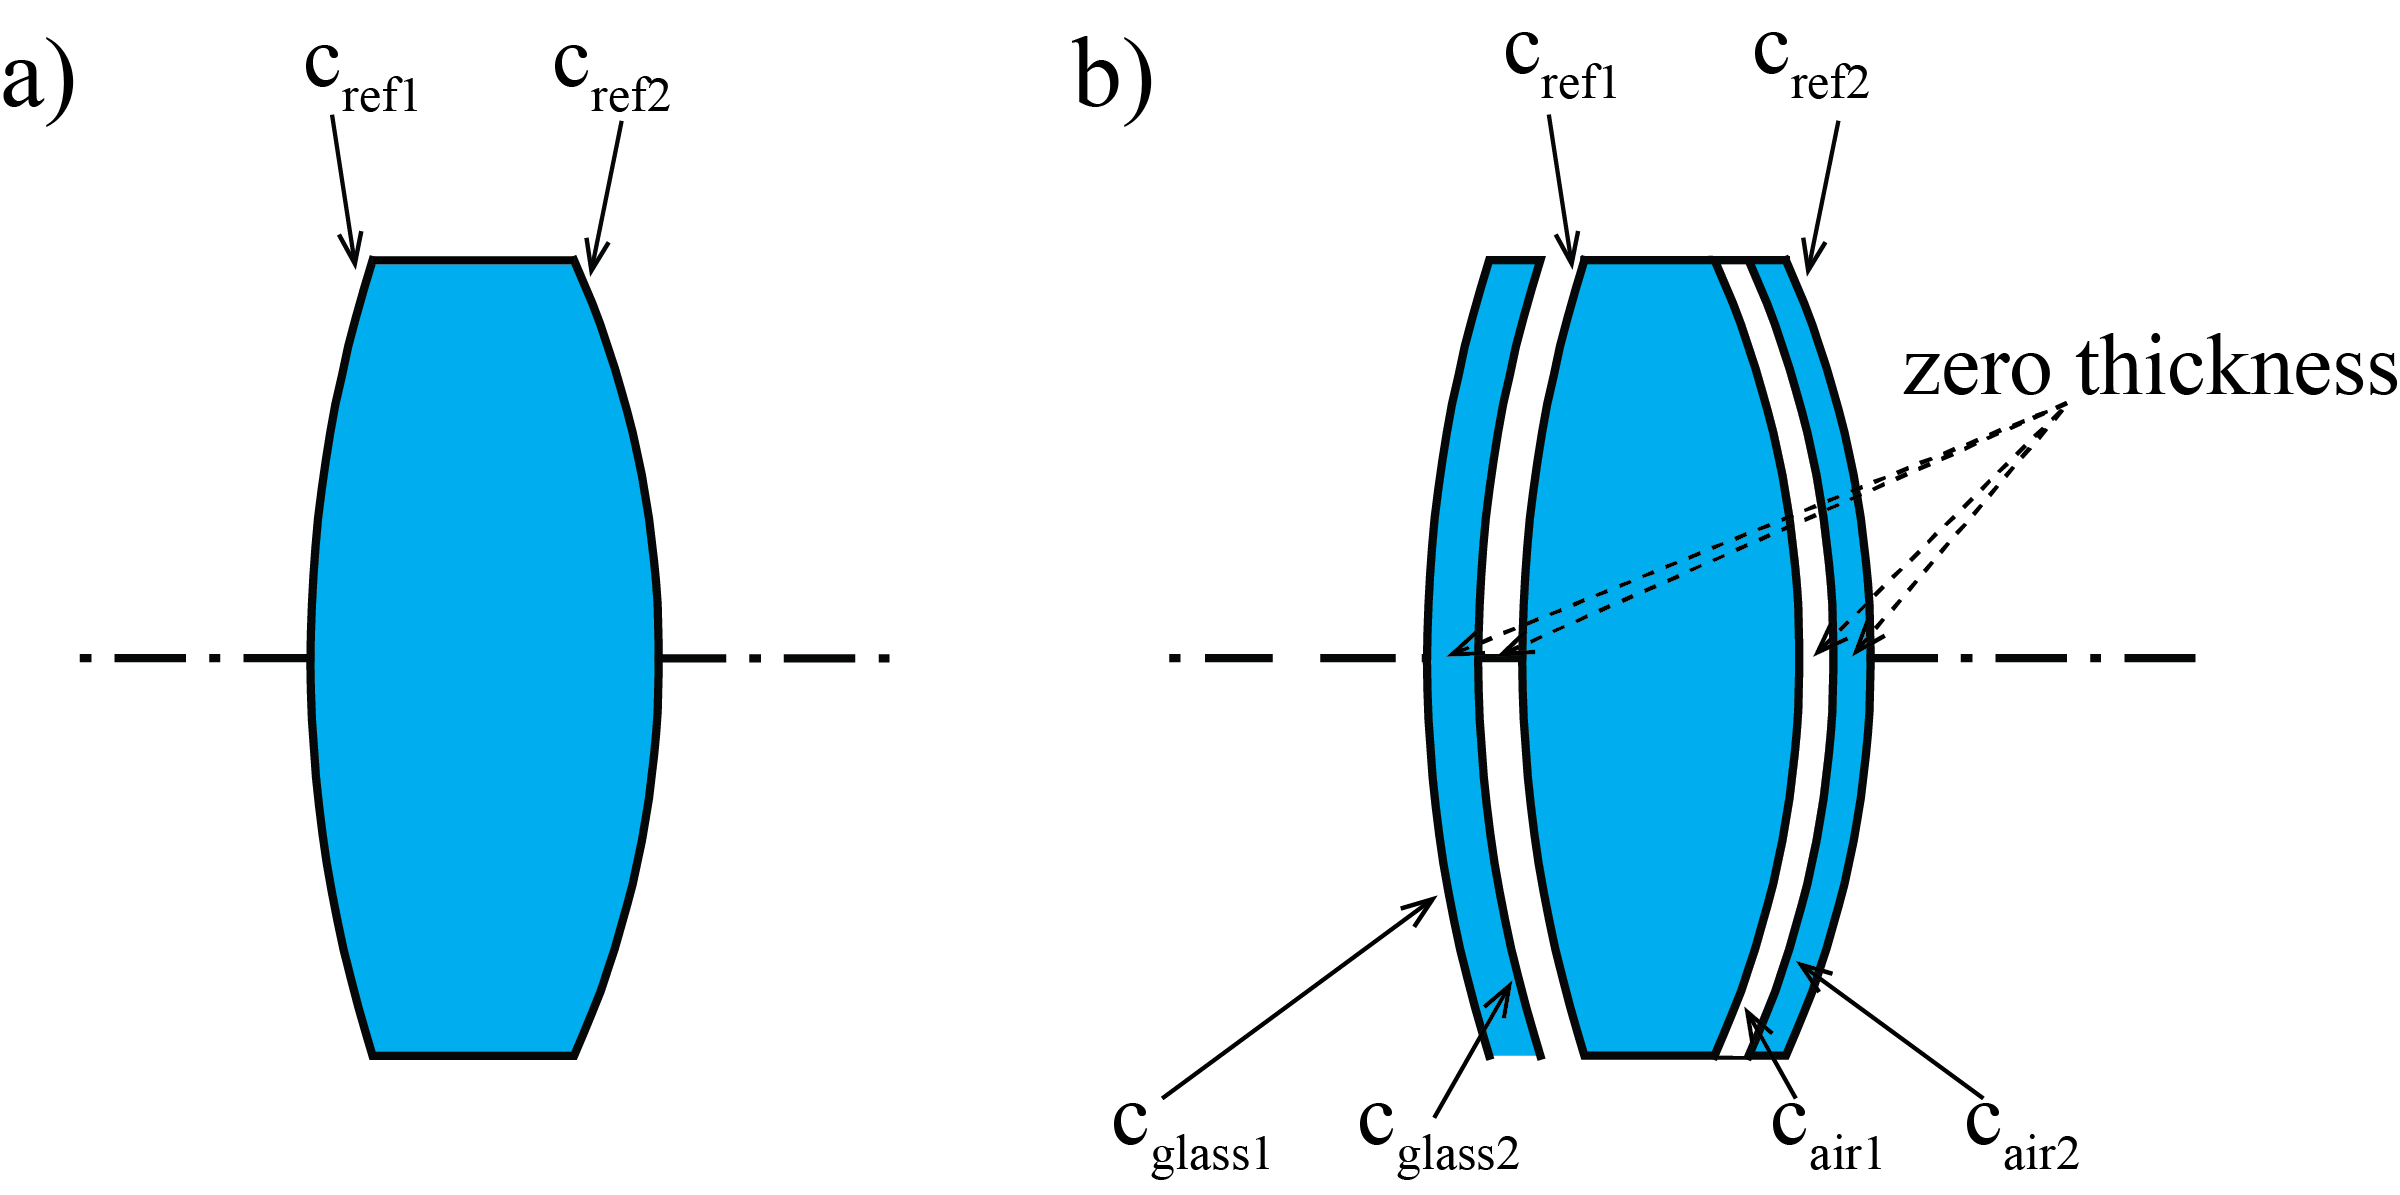
\includegraphics[scale=0.45]{chapter-2/figures/SPCS_illus.png}
    \caption{Illustration of the special version of SPC. a) A lens before adding any null element. b)  A glass null element has been attached to the surface on the left. An air null-element has been attached to the surface on the right. $c_{glass1} = c_{glass2} = c_{ref1}, c_{air1} = c_{air2} = c_{ref2}$. The speical version of the SPC usually adds one glass null element or one air null element. For demonstration purpose, different types of null elements are added to the lens, and the thickness of the null elements are also added.}
    \label{fig:SPCS-illus}
\end{figure}

Compared to the general version of the SPC, the special version is a rapid way to construct saddle point systems. However, the constructing positions are limited to the locations of the existing surfaces. As a result, some of the saddle points found by the general version can not be obtained by the special version of the SPC. In this research, the general version of the SPC is mainly used for acquiring new minima. When an SPC scan is performed on an existing surface, the saddle point constructed by the special version of the SPC can also be obtained. 

%%%%%%%%%%%%%%%\subsection{Saddle point construction intermediate}%%%%%%u%%%%%%%%

\section{Recommendations for applying Saddle Point Construction}\label{section: SPC recommendation}
As mentioned in the previous section, the SPC adds two extra curvatures to an existing optical system. It is straight forward, if the design goal is to add new elements to the system. Nevertheless, when applying the SPC in the practical design scenario, the technique can be used in different ways to achieve different design goals. Some scenarios are listed below as recommendations.

\subsection{Adding lens elements}
The direct way of applying SPC is to add a lens element to the existing system. This can be achieved by either inserting a glass null element or an air null element. Essentially, both approaches introduce two curvature variables to the system. Adding a glass null element can be treated as adding a lens element, while adding an air null element can be regarded as splitting an existing lens. The two approaches are described in the following two paragraphs.

\subsubsection{glass null element - adding a lens}
The Cooke triplet is chosen here as an example to demonstrate how SPC is applied. 
The position of the insertion of the glass null element is indicated by the dashed line in Figure \ref{fig:SPC-glass null element}. In principle, any position in the spaces between the lenses can be selected for the insertion. The choice of the position can be guided by the conventional lens design method. Examples of combining a traditional design method and the SPC method are given in Chapter 4.

In Figure \ref{fig:SPC-glass null element}, the insertion position is chosen between the middle lens and the right lens. As shown in the SPC scan curve, three zero-crossing points of the derivative of the merit function are found, hence three saddle points are found. Three new solutions with the added lens are listed in the same figure. Based on the scan curve, one would expect four solutions instead of three to be produced after optimizing from the three saddle points. It is the case when the minima are in the form of having an element with zero-thickness. However, when the thickness of the inserted element is increased, solution will disappear or merge with other solutions (an example is given in the next chapter in Figure \ref{fig:thicknesschange}). This is the situation in this example, and only three minima remained once the thickness is increased to a practical value. Among the three solutions, the added lenses present different optical powers. The original lens elements of the system remain almost the same powers compared to the status before insertion. In this example, two systems have better MF values (left system MF 43.27 $\mu m^2$, right system MF 47.80 $\mu m^2$) than the original one (MF 49.95 $\mu m^2$). The merit function used here is the default transverse-ray function in CODE V. It is a composite value, scaled so that it is the mean square of the weighted image radius.

\begin{figure}[h!]
    \centering
    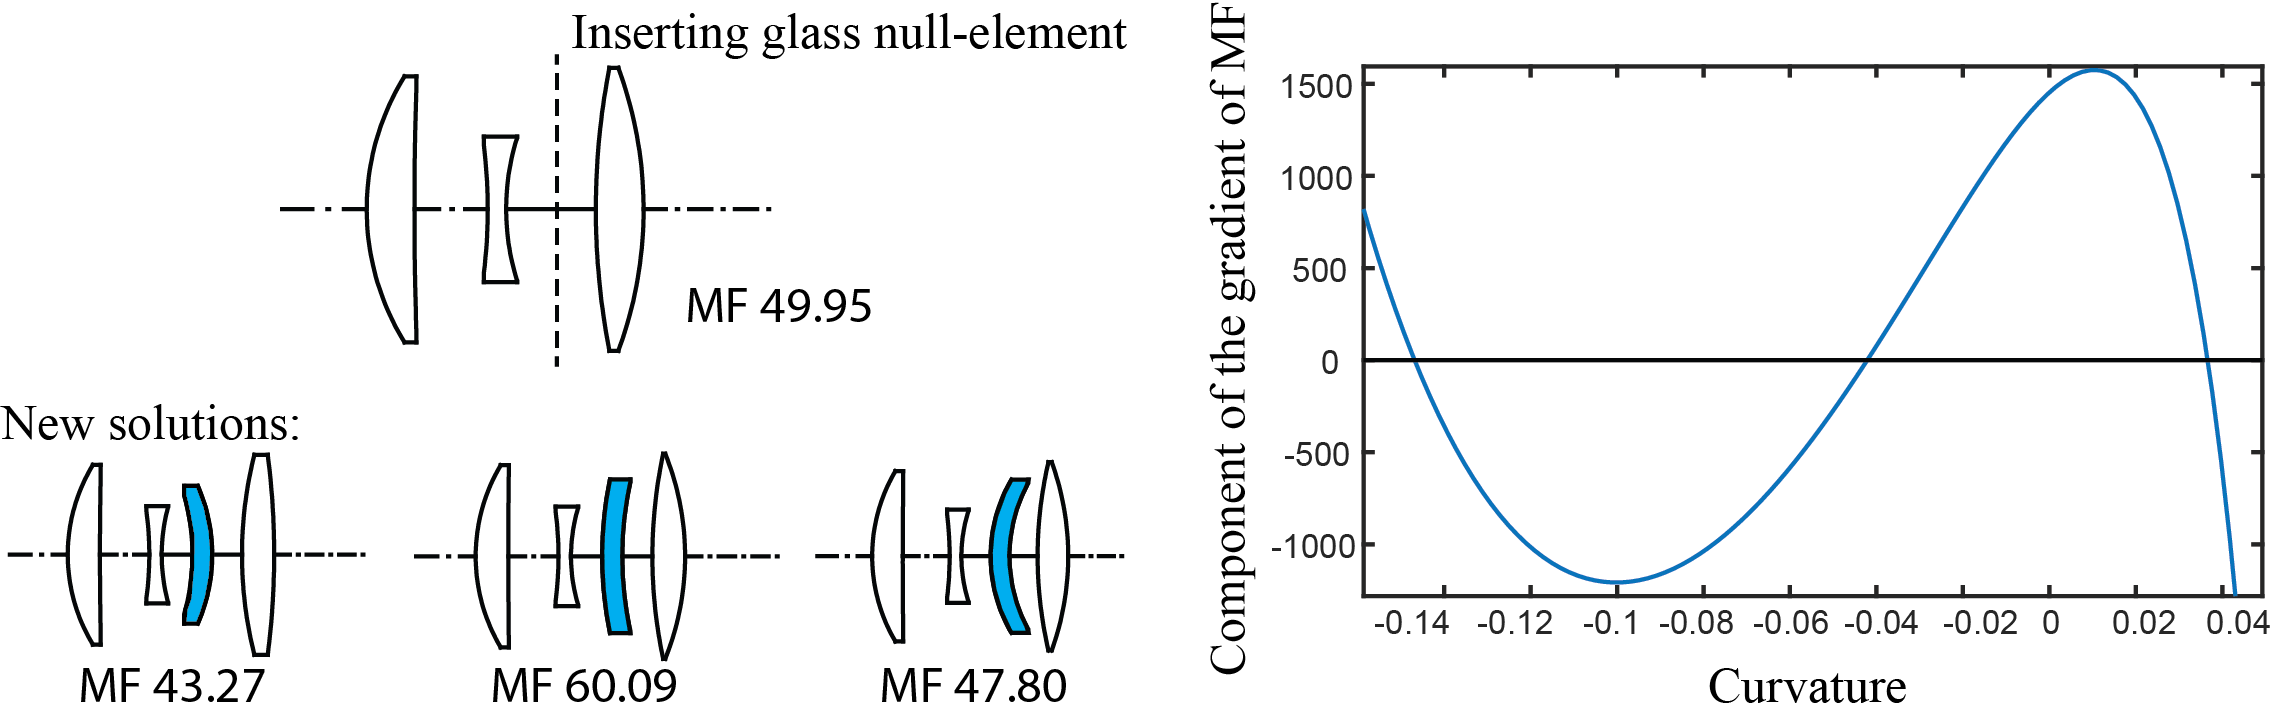
\includegraphics[scale=0.68]{chapter-2/figures/spc_add_glass.png}
    \caption{Adding lens element by adding glass null element using the SPC. The dashed line indicates the position where the null element is inserted. Three saddle points lead to four solutions with zero-thickness element (not shown). When the thickness of the inserted element is increased, three solutions with one lens more are obtained. The added lens elements are highlighted. MF values are listed for each system, and the unit is $\mu m^2$. }
    \label{fig:SPC-glass null element}
\end{figure}

\subsubsection{air null element- splitting a lens}

Alternatively, adding lenses can also be realized by splitting lenses. With the SPC, inserting an air null element into a lens is equivalent to splitting this lens. In Figure \ref{fig:SPC-air null element}, the most right lens element was chosen to be split. The dashed line indicates where the lens was split. The derivative as function of the curvature of the inserted air space is plotted in the right part of the figure. It is seen that there are four saddle points. Same as the situation in glass element insertion case, they lead to three solutions instead of five. The solutions and their merit function values are listed in Figure \ref{fig:SPC-air null element}. Evaluating the MF values, it is seen that three new systems all have better MF values than the original one. The inserted air spaces are highlighted.

Compared with the solutions produced by inserting glass null element, the solution on the right in Figure \ref{fig:SPC-air null element} for air null-element insertion presents a similar system shape as the solution on the left in Figure \ref{fig:SPC-glass null element} for glass null-element insertion. The similarity is shown by the same power distribution of each element in the systems. When adjusting the thickness and airspace, the two systems converge to the same solution. 


\begin{figure}[h!]
    \centering
    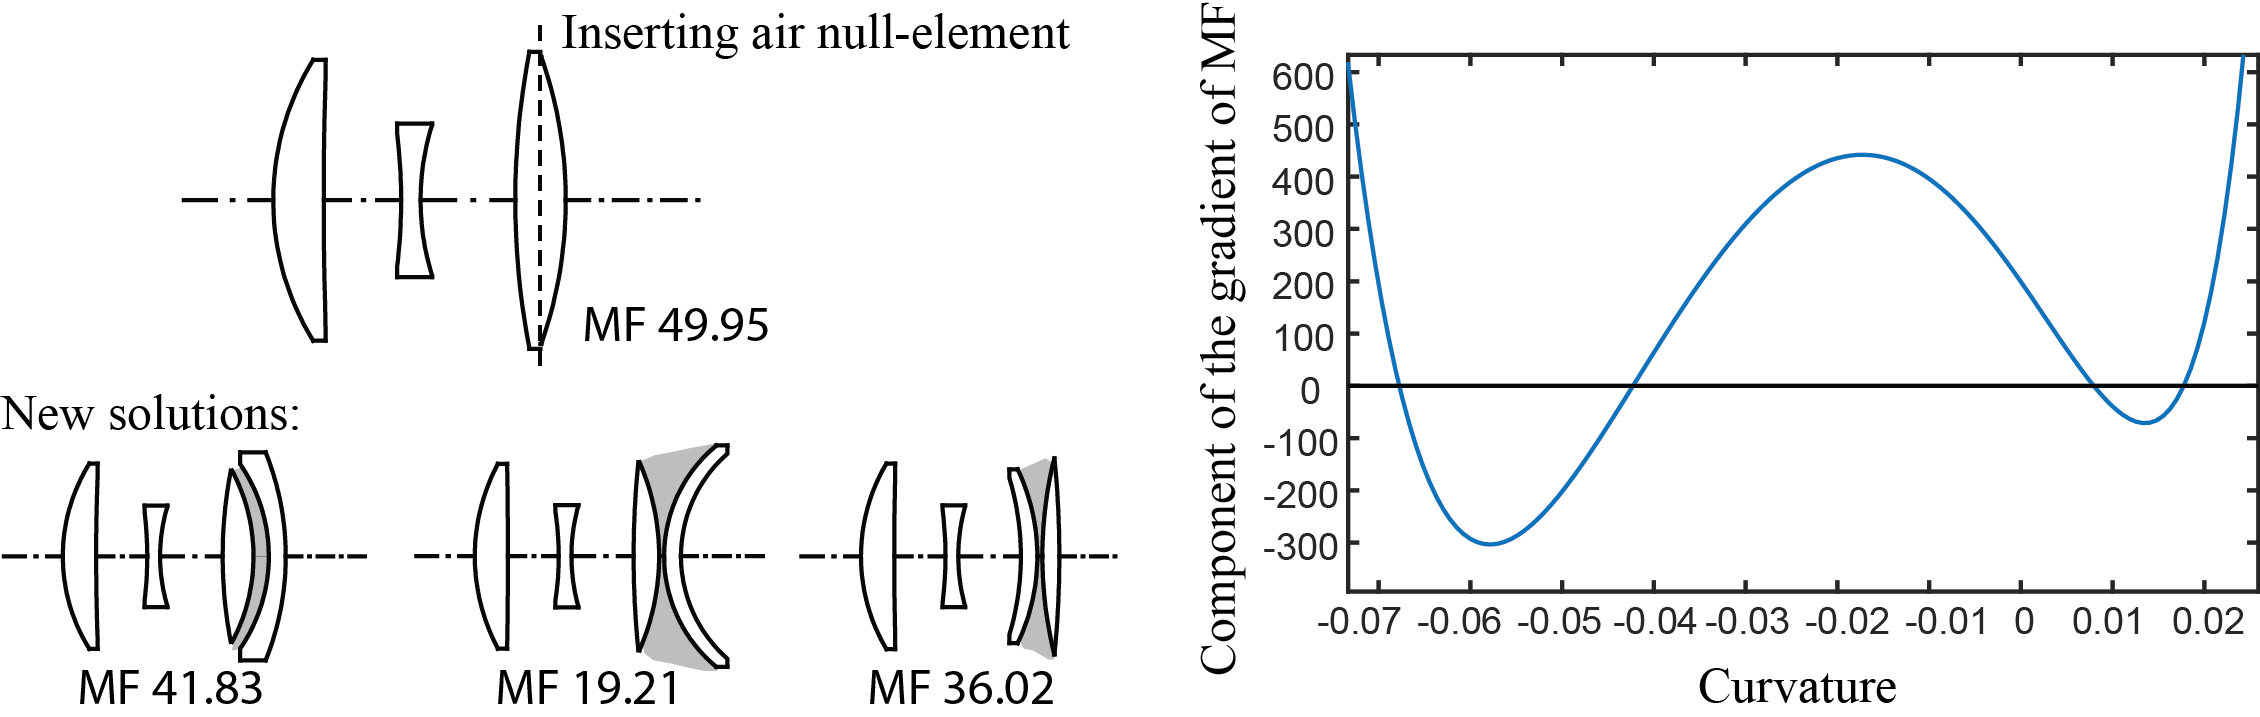
\includegraphics[scale=0.68]{chapter-2/figures/spc_add_air.png}
    \caption{Adding a lens element by adding an air null element using the SPC (splitting lenses). The dashed line indicates the SPC scan position. Four saddle points lead to three solutions with one lens more. The added air spaces are shaded. MF value of each system is listed, and the unit is $\mu m^2$. }
    \label{fig:SPC-air null element}
\end{figure}

\label{cp2-switching}
\subsection{Switching to alternative minima}

\subsubsection{The EXTRACT and ADD operation}
In practical lens design, it is usually important to obtain a better solution without changing the number of variables (lens elements). Adding extra elements in the system often means that the costs of the system become higher and that the system becomes less compact. 

When using the SPC, with some subsequent steps described below, it is possible to switch between local minima with the same number of variables. Illustrated in Figure \ref{fig:SPC-switch-example}, the first step is to choose which lens to modify. The middle one of the Cooke triplet was chosen in this example. The next step is to extract this element from the original system as follows. The thickness of the chosen element is gradually reduced to zero while in each step the system is optimized with respect to the remaining variables. Small steps should be applied for the change of the thickness to prevent the optimization moving to a different basin of attraction. When the basin of attraction of the optimization changes, a sudden change in the merit function value can be observed. After the thickness is reduced to zero, the curvatures of the two surfaces are usually different. Next the curvatures can be changed gradually until they become equal and the system is optimized with respect to the remaining variables after each step. 

\begin{figure}[h!]
    \centering
    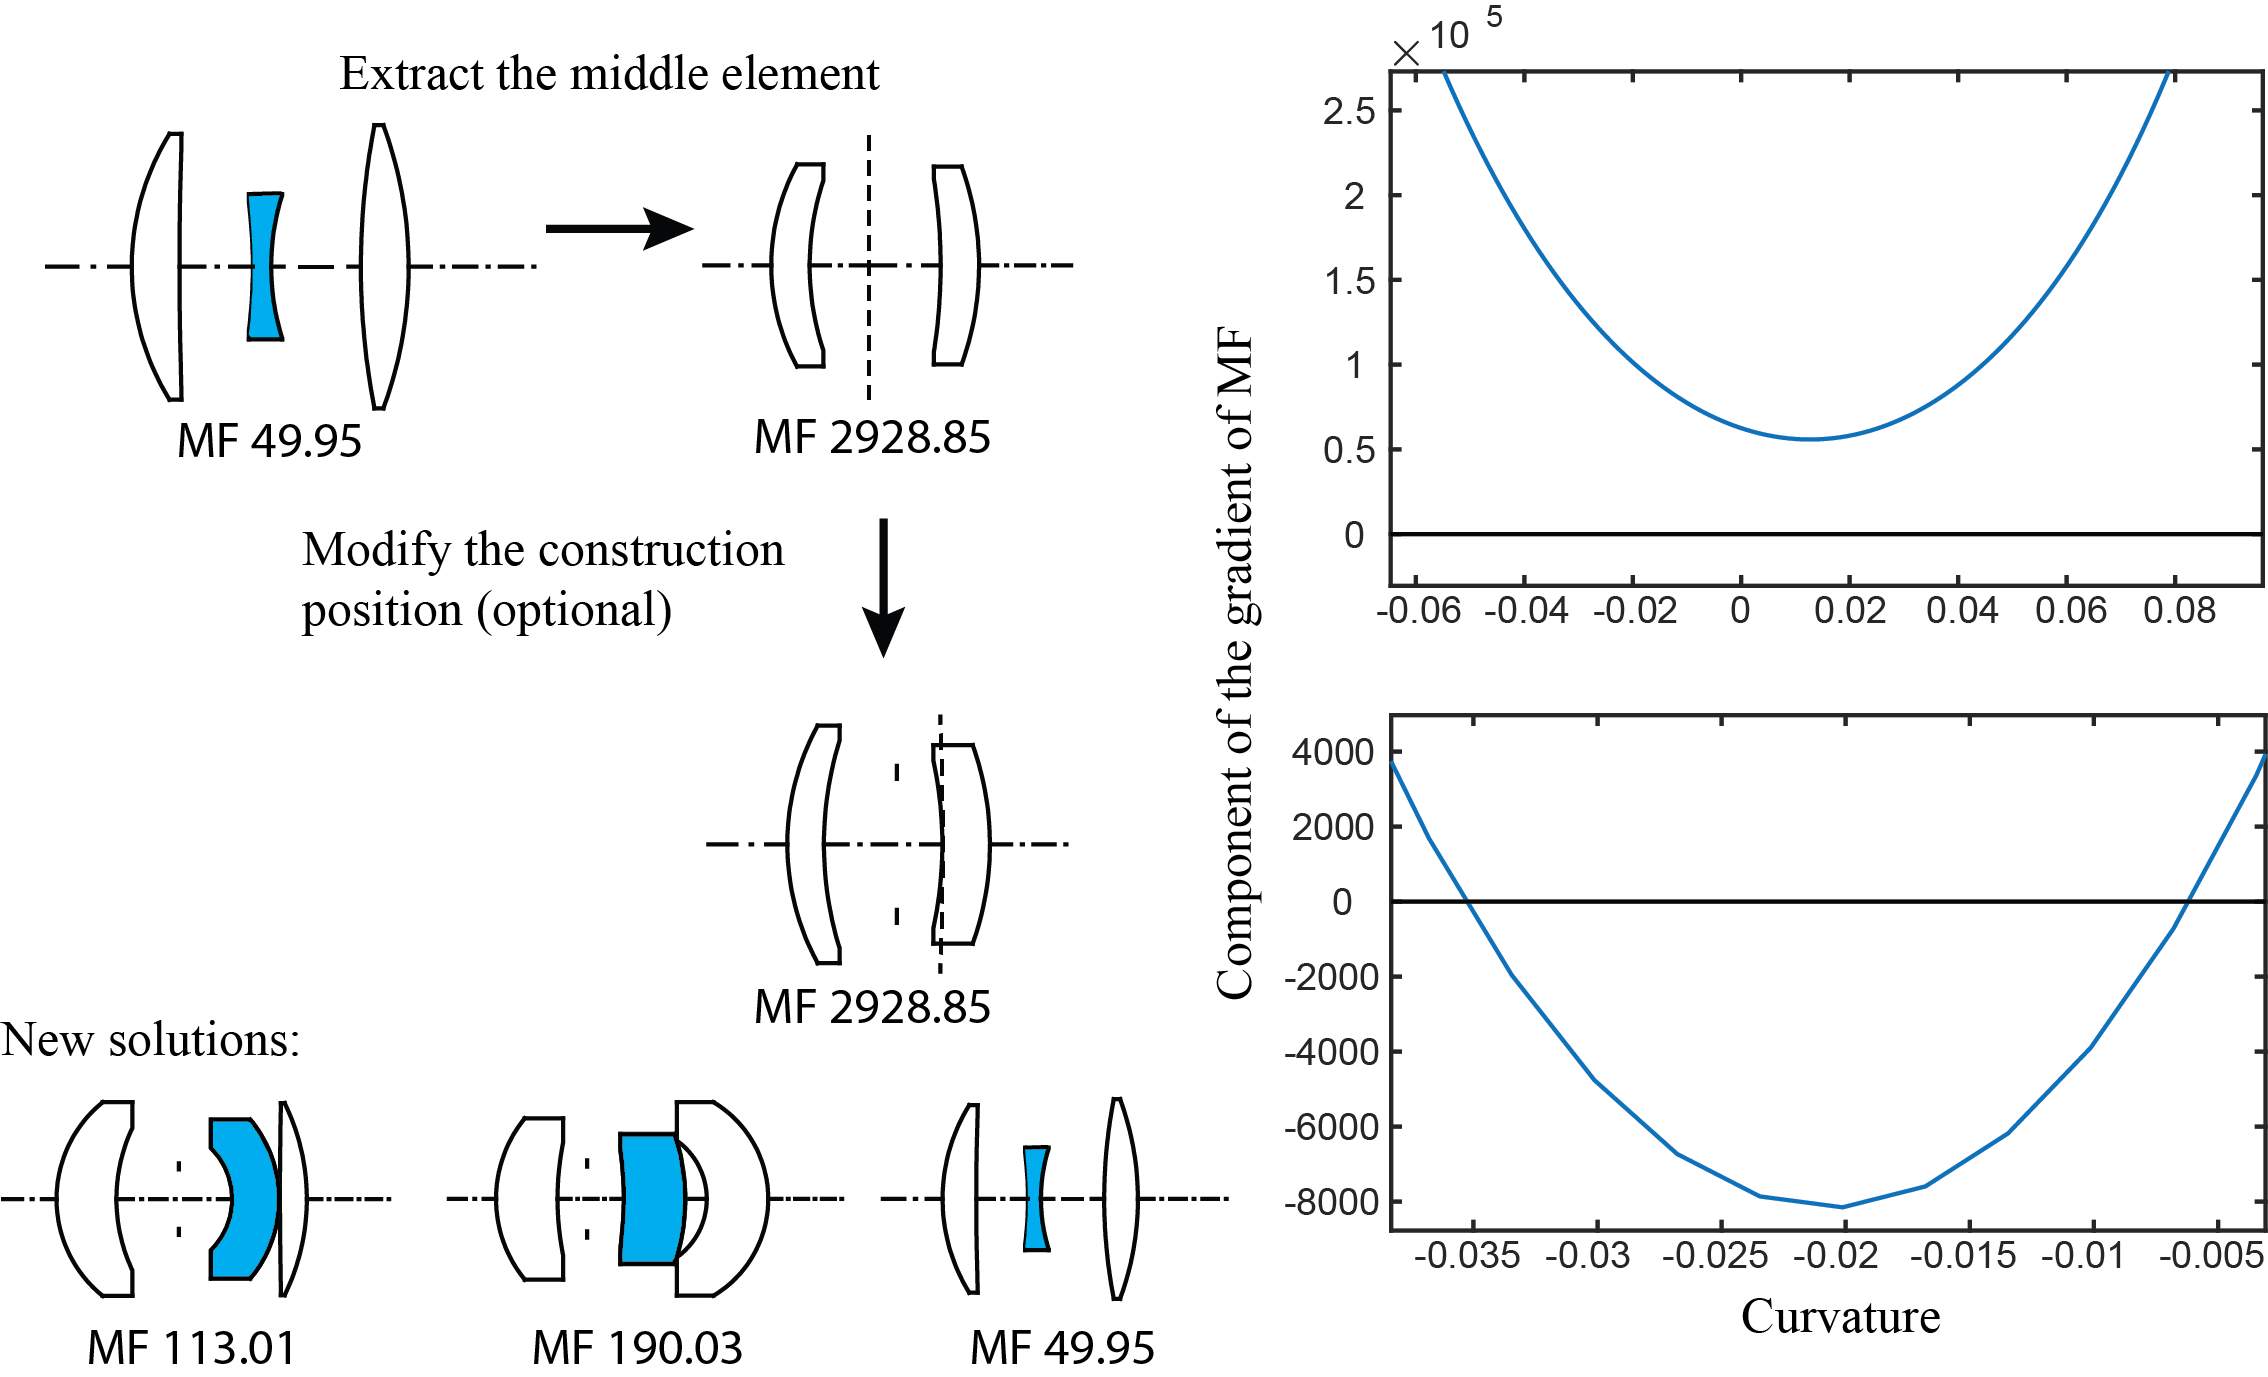
\includegraphics[scale=0.68]{chapter-2/figures/spc_switch.png}
    \caption{Switching to different solutions with the SPC. The middle lens element was chosen to be first extracted, and the SPC was performed at the same location. However, no saddle point was found in that location. The scanning location was then shifted right. Two saddle points and three solutions were obtained. MF value of each system is listed, and the unit is $\mu m^2$. }
    \label{fig:SPC-switch-example}
\end{figure}

Once the thickness of the chosen lens has been made zero and the two curvatures have been made equal by this procedure, the null element can be extracted from the system without changing the value of the merit function. In fact, we have now a system with one lens less which is a local minimum for the reduced number of variables. The system is ready to be inserted with null element in order to add back the extracted lens and obtain new local minima. The null element is usually inserted at the same location where the lens is extracted and the derivative of the merit function with respect to the curvature is scanned to search for saddle points. In Figure \ref{fig:SPC-switch-example}, the curve plot on the top shows the SPC scan when it is performed at the position of the extraction. It is seen that the scan shows no saddle point. The subsequent step is to change the position where the null elements is inserted in the space between the two lens elements. Where the arrow points down in Figure \ref{fig:SPC-switch-example}, the position of the insertion of a null element is chosen to coincide with the left surface of the right lens. The curve of the derivative has two zero-crossings, which indicates two saddle point systems. One of the saddle points can be explained by the special version of the SPC \cite{BociortSPCSexplained}, where the curves of the inserted element are identical to the surface which the null element is attached to. 

Three solutions were obtained from the two saddle points. After relaxing all variables and optimizing, the solution on the right in Figure \ref{fig:SPC-switch-example} becomes identical to that of the original Cooke triplet. The other two solutions are new solutions. None of the two shows better MF values compared to the Cooke triplet design. 


\subsubsection{The ADD and EXTRACT operation }
It was shown that with an extract-and-add strategy one can switch systematically from one local minimum to other minima, with the same number of variables. A intermediate step is necessary to first reduce the number of the variables in the original problem (by extracting a lens). 

It is also possible to switch to different solutions using the SPC by first increasing the number of variables: an add-and-extract strategy. However, it is not really recommended since it requires more decisions on where to add or extract in the intermediate steps. For an extract-and-add strategy, it is demonstrated in the previous section that the designer only needs to decide where to extract an element. In contrast, an add-and-extract strategy will work as follows: the designer first has to decide where to add an element to the original system. Then, after the SPC operation, usually more than one solution is produced. In the simplest case, the designer can decide to extract the same element for all of them. However, it is also possible to decide to extract different elements from the solutions obtained after SPC. In either way, the add-and-extract strategy will require more decision steps than the extract-and-add strategy.

%\subsection{Derivatives base on the technique provided}
\section{Conclusion}
In this chapter, the Saddle Point Construction (SPC) method is explained in detail. The method constructs saddle point system with Morse Index $1$ in a higher dimensional space (from dimension $N$ to dimension $N+2$). Optimizing from a saddle point of Morse Index $1$ can systematically lead to two local minima. The general version of the SPC involves a scan of the inserted curvatures to search for the saddle point. It is not guaranteed that the scan will generate saddle points. In the special version of the SPC a null element attached to an existing surface is added, where a saddle point system can be immediately obtained \cite{BociortSPCSexplained}. 

By performing a scan to find systems where the first order derivative of the merit function vanishes, the general version of SPC usually finds more than one saddle point, therefore, often several solutions are obtained. When such a scan of the derivative happens at a position same as an existing surface, the saddle point predicted by the special version of the SPC will also be included. 

Recommendations on how to use the SPC in practice are provided: an SPC scan can be done either by scanning a glass null element (adding a lens element) or scanning an air null element (splitting a lens element).  Depending on the scan positions, the two approaches can produce similar solutions ( e.g. Figure \ref{fig:SPC-glass null element} and Figure \ref{fig:SPC-air null element}).

Switching to different local minima using the SPC without increasing the number of elements (ie. variables), can be very useful. This is realized by first extracting a lens element, and then performing an SPC scan at the extracted position. Figure \ref{fig:SPC-switch-example} demonstrates the steps where extra solutions are obtained. 

In the following two chapters, the SPC is used in the way described in this chapter. A detailed study of the saddle point - minima networks using SPC is presented in Chapter 3. Several practical examples are given in Chapter 4 demonstrating how these approaches can be used in lens design. 


\references{dissertation}



%% Use letters for the chapter numbers of the appendices.
\appendix

%\include{appendix-a/appendix-a}

%% Turn off thumb indices for unnumbered chapters.
\thumbfalse

\chapter*{Summary}
\addcontentsline{toc}{chapter}{Summary}
\setheader{Summary}

In this thesis, we explore how lens design and optimization techniques can adapt to the design (optimization) space in order to increase the lens design efficiency. 

The optical lens design space is known to be very complicated. This is a high-dimensional space defined by the degrees of freedom and the quantified performance of a parameterized optical system. This space is also nonlinear which means there are multiple local minima (you can think of the bottom of a crater in the geological landscape) with different values. In modern optical lens design, the task can be described as searching for the global minimal value in the high-dimensional space. For sophisticated lens designs, the number of the degrees of freedom increases in order to gain more control of the design. It brings two major difficulties:  
\begin{enumerate}[nosep]
\item The size of the high dimensional space increases according to the power law which means a brute force search is practically impossible. 
\item The number of local minima increases with the number of the degrees of freedom used. It indicates the number of undesired local minima becomes larger. Hence, the difficulty of finding best minima also increases.  


\end{enumerate}

% technique has been developed 
Over the past decades, different design and optimization techniques have been examined on their effectiveness of obtaining a global optimal solution. Some of the techniques have been integrated into commercial lens design software. However, these algorithms are based almost exclusively on generally applicable mathematical models and use little or no specific knowledge about the optical system (and its design landscape). As a result, little information is available on how these techniques should be used in a practical design task instead of implementing them as a lottery draw. 

We emphasize in this thesis that, considering an actual lens design process, the design space is not only statically complicated, but also dynamically changes through the design process. The dynamic aspect affects the design landscape. As a consequence, the number of local minima and the effectiveness of the optimization techniques can be impacted. In Chapter \ref{chapter_5_SMS}, a study using Simultaneous Multiple Surface (SMS) method as one of the design strategies, compares the effectiveness of different strategies under static and dynamic design landscape.

Saddle Point Construction (SPC) is a design method which can rapidly construct saddle points with Morse Index 1 in a design space. These saddle points serve as agents to guide the local optimization to obtain new minima. Different from other optimization techniques, it also reveals a special structure in the lens design landscape: certain saddle points existing in the landscape are reducible to minima of simpler systems plus one additional lens element.

Previous research shows potentials of SPC as a systematic lens design technique. In this thesis, we further examine the practicality of SPC as a global optimization and semi-global optimization (to generate a small pool of solutions) tool. The dynamic aspect of the design space is particularly of interest since it is relevant to an actual design practice. 

To assess the robustness of SPC as a global optimization method, we examine the solution network of saddle points and minima for several scenarios. We formulate three falsifiable research questions and have falsified two of them based on the observations:
\begin{enumerate}[nosep]
\item In a lens design landscape, are all the saddle points able to be constructed using SPC? The answer to this question is no. The detail of the analysis is given in Chapter \ref{chapter_SPC_simple_system_landscape}.
\item Are all the minima always linked via the saddle point - minima network revealed by SPC? The answer to this question is also no. The analysis is provided in Chapter \ref{chapter_SPC_simple_system_landscape} and also supported by the wide-angle lens example in Chapter \ref{chapter_4_complex_system_exploration}.
\item Does the saddle points - minima network obtained via SPC always contain the best or the best pool of solutions for lens design? We cannot give an answer to this question. However, in the examples we have examined, the positive side of this question is valid. 
\end{enumerate}

Despite the fact that using SPC does not guarantee capturing all the local minima in the design space, we observe that the good minima are always captured in our examples. Given its systematic way of obtaining local minima, we consider it as a useful global search technique for lens design. 

In addition, in Chapter \ref{chapter_4_complex_system_exploration}, we demonstrate that SPC can be particularly effective for complicated systems when the goal is to get a small pool of solution candidates while the system configuration is not drastically changed. 

\begin{comment}
At last, we provide our thoughts on how the lens design landscape can be further studied. However, it is not straightforward how it can be related to an everyday design task. We believe that a tool gets improved during its practice, therefore, suggestions on further making SPC as a practical lens design tool are also given at the end. 
\end{comment}


\begin{comment}
We analyze the characteristics of the optical lens design space. We emphasize its dynamic property, which means the landscape changes given different design condition is changed, which is a common thing during the design practice

This dissertation addresses the typical problem during optical design or generally all engineering problem -- how to find the best solutions in a parameterized system. 

Goal/Nature of the problem: find the best solution -> assess whether the solution is sufficient or not, if it is not, the process should go to the next design decision; if it is sufficient, the solution can be taken. 

How: Parameterize the system with the multiple variables with a model representing its physical property therefore the performance can be evaluated.  
Given the model, use mathematical tools to optimize in order to get the best solution.
(alternatively, you can realize this by continuous testing and modifying during your manufacture -> caveman's method)

  Sub-problem statement: after parameterization, the optimization space of the system is usually a non-convex space, which indicates a presence of multiple local minima when a typical local optimizer is used. Situation of non-convex space provides difficulties in getting a satisfactory solution: it is difficult to find all the existing solutions in the design space. With incomplete set of information, the following question exist: will there be a better solution if one keeps searching given the current system configuration. As a results, techniques that can quickly generate new solutions given a design configuration is welcome to verify if a better system can be found. The process usually ends when a good enough result is found or a time limit is reached. 

Goal: Find whether there is a better solution in a non-convex optimization problem. This is global optimization. 

How: 
1) starting from a very good starting point (this indicates good technique is needed to construct the starting points) and after arriving at a local minimum, GO technique is used to check whether better solutions can be found (the anticipation is not). 

2) starting from somewhat working point (this indicates small effort to determine the starting point) and combined with GO technique to see if we could find more better solutions. The anticipation is that there would be some better results appear. 

    Sub-problem statement: SPC is a GO technique. SPC shows systematic approach and reveals certain structure between optimization landscape and the optical design model. The following questions are interesting regarding SPC:
1) How SPC is performing as a GO technique? In terms of the completeness and efficiency for finding new solutions. Completeness -> do I find every solution, or at least all solutions find by other algorithms.  Efficiency-> what is the time needed to run such GO. Is it a limited amount of algorithmic trial?
2) Does it show more profound connection to the lens design problem such that it could be used to facilitate the design more? This question should be implicitly included in the first one. It is more of scientific curiosity that if the nature of SPC is connected to the lens design problem. 

    Sub-problem statement: SMS is a starting-point-generating technique. The hypothesis is that it generates a good starting point since the method is guided by the physical rules (Fermat's Principle). Is SMS method the method that providing the starting point that close to the best local minimum (via one local optimizer)? 
    
To sum, it is the balance between the effort of getting a good starting point and running less optimization. SPC as an optimization technique needed to be investigated for its GO efficiency. It means, given a non-perfect starting point, the GO method is preferred to efficiently find the best solution. Chapter 2-4 is trying to clarify this.
SMS as a technique to construct starting points, the ultimate question is that if it constructs the starting point that the minimum optimization effort it needed. Chapter 5 is trying to answer this question. 
\end{comment}
\chapter*{Samenvatting}
\addcontentsline{toc}{chapter}{Samenvatting}
\setheader{Samenvatting}

{\selectlanguage{dutch}

Samenvatting in het Nederlands\ldots

\noindent geschreven worden ...

}


\chapter*{Curriculum Vit\ae}
\addcontentsline{toc}{chapter}{Curriculum Vit\ae}
\setheader{Curriculum Vit\ae}

%% Print the full name of the author.
\makeatletter
\authors{\@firstname\ {\titleshape\@lastname}}
\makeatother

\noindent
\begin{tabular}{p{4\parindent}l}
    20-03-1988 & Born in Nei Mongol, P. R. China 
\end{tabular}

\section*{Work Experience}
\begin{tabular}{p{4\parindent}l}
    2019--Now & YieldStar Application, ASML (Eindhoven, the Netherlands) \\

    \\
\end{tabular}

\section*{Education}
\begin{tabular}{p{4\parindent}l}

    2013--2018 & PhD Candidate \\
    & Delft University of Technology (Delft, the Netherlands)\\
    & Datalogic (Bologna, Italy, Jan--May, 2016)\\
    & Polytechnic University of Madrid (Madrid, Oct--Dec, 2015)\\
    \\
    2011-2013 & Master Applied Physics \\
    & Erasmus Mundus OpSciTech (Optical Science and Technology)\\
    &Delft University of Technology (Delft, the Netherlands, 2012--2013)\\
    &Warsaw University of Technology (Warsaw, Poland, 2011--2012)\\
    \\
    2007--2011 & Bachelor Optical Engineering\\
    & Zhejiang University (Hangzhou, P. R. China)
    
\end{tabular}
    
\begin{comment}
\begin{tabular}
    %% The width of the second column is the width of the page, minus the width
    %% of the first column (4\parindent) minus four times the separation between
    %% the start of the column and its contents.
    \begin{minipage}{\textwidth-4\parindent-4\tabcolsep}
        %% We divide the minipage 20/80.
        \begin{tabular}{@{}p{0.2\linewidth}@{}p{0.8\linewidth-\tabcolsep}}
            \textit{Thesis:} & Eine neue Bestimmung der Molek\"uldimensionen \\
            \textit{Promotor:} & Prof.\ dr.\ A.\ Kleiner
        \end{tabular}
    \end{minipage}
\end{tabular}
\end{comment}
\begin{comment}
\section*{Awards}

\begin{tabular}{p{4\parindent}l}
    1922 & Nobel Prize in Physics \\
    \\
    1925 & Copley Medal \\
    \\
    1929 & Max Planck Medal \\
    \\
    1999 & Time magazine's person of the century
\end{tabular}
\end{comment}

\chapter*{List of Publications}
\addcontentsline{toc}{chapter}{List of Publications}
\setheader{List of Publications}
\label{publications}

%% We use the 'etaremune' environment (the reverse of 'enumerate') to get a
%% numbered list of publications in reverse chronological order. If the list of
%% authors is long, it might be useful to emphasize your own name with \textbf.
\Large{\textbf{Refereed publications}}

\begin{enumerate}\small{
\item \textbf{Z.\ Hou},  M. Nikolic, P. Benitez, and F. Bociort, "SMS2D designs as starting points for lens optimization," \href{https://doi.org/10.1364/OE.26.032463}{\textit{Opt. Express} \textbf{26}, 32463-32474 (2018)}.
\item \textbf{Z.\ Hou}, I. Livshits, and F. Bociort, "One-dimensional searches for finding new lens design solutions efficiently," \href{https://doi.org/10.1364/AO.55.010449}{\textit{Appl. Opt.} \textbf{55}, 10449-10456 (2016)}. 
\item A. Reyes-Reyes, \textbf{Z.\ Hou}, E. van Mastrigt, R. C. Horsten, J. C. de Jongste, M. W. Pijnenburg, H. P. Urbach, and N. Bhattacharya, "Multicomponent gas analysis using broadband quantum cascade laser spectroscopy," \href{https://doi.org/10.1364/OE.22.018299}{\textit{Opt. Express} \textbf{22}, 18299-18309 (2014)}.
}\end{enumerate}

\vspace{3mm}
\noindent
\Large{\textbf{Conference proceedings}}
\begin{enumerate}\small{
\item \textbf{Z.\ Hou},  I. Livshits, and F. Bociort, "Practical use of saddle-point construction in lens design," \href{https://doi.org/10.1117/12.2312494}{\textit{Proc. SPIE} \textbf{10690}, Optical Design and Engineering VII, 1069007 (2018)}.
\item \textbf{Z.\ Hou} and F. Bociort, "Reducible complexity in lens design," \href{https://doi.org/10.1117/12.2191364}{\textit{Proc. SPIE} \textbf{9626}, Optical Systems Design 2015: Optical Design and Engineering VI, 96260J (2015)}.
\item I. Livshits, \textbf{Z. Hou}, P. van Grol, Y. Shao, M. van Turnhout, P. Urbach, and F. Bociort, "Using saddle points for challenging optical design tasks," \href{https://doi.org/10.1117/12.2061975}{\textit{Proc. SPIE} \textbf{9192}, Current Developments in Lens Design and Optical Engineering XV, 919204 (2014)}.

}\end{enumerate}

\vspace{3mm}
\noindent
\Large{\textbf{Conference contributions}}
\begin{enumerate}\small{
\item \textbf{Z. Hou}, Y. Zhang, and F. Bociort, "Design Using Saddle Point Construction in Complex Lens Systems," oral presentation at the European Optical Society Biennial Meeting, Delft, the Netherlands (October 2018).
\item \textbf{Z. Hou}, I. Livshits, and F. Bociort, "Practical use of saddle-point construction in lens design," oral presentation at the SPIE Optical Systems Design conference, Frankfurt, Germany (May 2018).
\item \textbf{Z. Hou}, "One-dimensional searches for finding new lens design solutions efficiently,"  Excellent Oral Presentation Award at the International Doctoral Students Conference on "Opportunities and Challenges Arises from Global Technological Revolution", Zhejiang, China (May 2017).
\item \textbf{Z. Hou}, F. Bociort, I. Livshits, and H.P. Urbach, "A systematic study on the design landscape of a pin-hole lens," oral presentation at the 10th International Conference on Optics-photonics Design and Fabrication, Weingarten, Germany  (March 2016).
\item \textbf{Z. Hou}, F. Bociort, and I. Livshits, "Reducible complexity in lens design - 
replacing high-dimensional search by one-dimensional searches to find new solutions efficiently," poster presentation at the IST Science Day, Delft, the Netherlands (October 2015).
\textbf{Z. Hou} and F. Bociort, "Reducible complexity in lens design," invited Paper at the SPIE Optical Systems Design conference, Jena, Germany (September 2015). 
\item F. Bociort, P. van Grol, I. Livshits, \textbf{Z. Hou}, Y. Shao, P. Urbach, "Saddle-point methods for systematic design," the European Optical Society Biennial Meeting, Berlin Adlershof, Germany (September 2014).
I. Livshits, \textbf{Z. Hou}, P. van Grol, Y. Shao, M. van Turnhout, P. Urbach, and F. Bociort, "Using saddle points for challenging optical design tasks," the SPIE OPTICAL ENGINEERING + APPLICATIONS conference, San Diego, U.S.A. (August 2014).

}\end{enumerate}


\end{document}

